%!TEX root = ../iotpaper.tex

\section{Project Proposal}
\label{sec:Proposal}

In an \gls{IoT} environment, mobile devices may need to pair or authenticate themselves to other devices. However, unlike the traditional internet, an \gls{IoT} environment does not typically have a centralized certificate authority, making it difficult for one device to determine if another device is authentic. Furthermore, these \gls{IoT} devices are often resource-constrained, meaning traditional cryptographic defenses that support confidentiality, integrity, and authenticity difficult to implement \cite{cisco:iot-pf,authmodels}.

One potential solution to this problem is to use biometrics---especially motion and gestures---in order to validate the identity of the device. Prior work has shown that impostors has a low probability of imitating a gesture calibrated to another person successfully \cite{Casanova}. Furthermore, motion recognition is suitable for \gls{IoT} systems which feature small sensors and low powered devices because motion recognition can achieve high accuracy with just an accelerometer \cite{RuizeXu}. 

Some prior work have looked at motion sensor data fusion across different devices to detect pairing, for example detecting device collision when tiling two tablets together \cite{SyncGes}. Existing work in gesture recognition and event detection focuses on gestures on the same device or similar devices (e.g. two tablets, gestures on a Wiimote \cite{LiuuWave}). However, pairing in an \gls{IoT} environment is usually needed for two asymmetric devices with different types of hardware sensors (e.g. a smartwatch with a smartphone).

In this project, we propose to analyze the use of gestures as a biometric for peer-to-peer authentication in an \gls{IoT} scenario, where sensor devices are asymmetric. 
Our project will analyze the following three key defense models for authentication.

\begin{itemize}
\item \emph{Model 1:} This system model contains three entities: a legitimate prover, a verifier, and an attacker. The legitimate prover is non-malicious and wants to pair with the verifier. Both the legitimate prover and the verifier are owned by the same person (e.g. a smartphone and a smartwatch). However, the attacker is a malicious prover and wants to also pair with the verifier. To distinguish between the attacker and legitimate prover, the verifier uses gesture recognition to distinguish between the two parties. 

\begin{figure}[!tb]
\centering
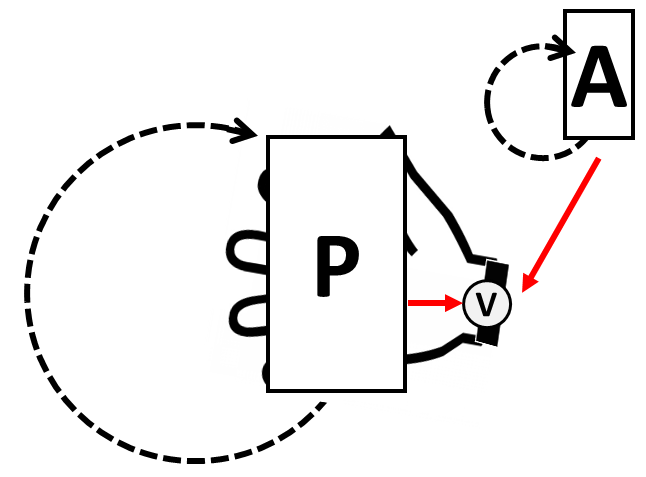
\includegraphics[width=0.65 \linewidth]{./figures/model1.png}
\caption{System model for defense model 1. The verifier (V) and the prover (P) are synchronized in motion. The attacker (A) must try to mimic the motion of the verifier in order to trick the system.}
\label{fig:Model1}
\end{figure}

Since the legitimate prover and verifier are owned by the same person, the user performs any generic gesture while holding both devices as shown in \autoref{fig:Model1}. Accelerometer data is used to read the gesture, and a matching gesture authenticates the prover.

In contrast, the attacker must mimic the gesture of the verifier in order to trick the verifier. Our hypothesis is that we can keep false negatives (rejecting legitimate provers) and false positives (accepting attackers) to less than 10\%. This is modest compared to existing works due to the hardware asymmetry.  

% To pair two devices together, the devices simultaneously measure the motion with the accelerometer. If the data matches, then the devices successfully pair. An attacker for this system tries to impersonate a gesture that the verifier is using.

\item \emph{Model 2:} This system model contains the same three entities as in Model 1. In this model, the verifier has previously calibrated a single secret gesture with the user that is needed to pair with the device as shown in \autoref{fig:Model2}. Devices that want to pair with the verifier must produce accelerometer data that matches this gesture with no prior knowledge about the gesture. Since this gesture is a predefined secret, only the prover needs to collect accelerometer data during the proof of authenticity.

\begin{figure}[!tb]
\centering
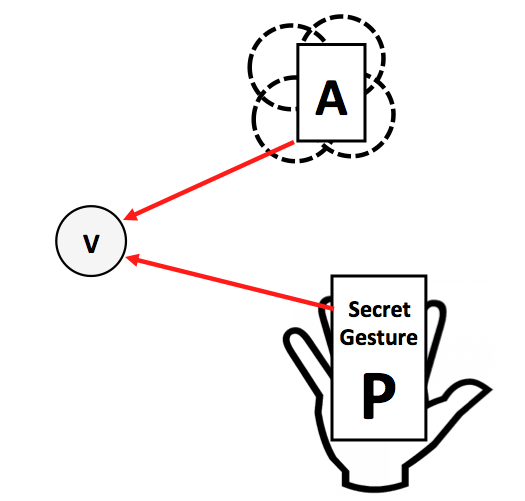
\includegraphics[width=0.6 \linewidth]{./figures/model2.png}
\caption{System model for defense model 2. The verifier (V) and the prover (P) are not synchronized in motion, and the verifier has previously established a secret gesture for pairing. The attacker (A) can brute force a gesture if it has no knowledge of the secret gesture, or it may imitate a gesture that it sees that a legitimate prover used.}
\label{fig:Model2}
\end{figure}

An attacker may try to trick this model in the following two ways. First, if no information about the secret gesture has been leaked to the attacker, it will attempt a brute force attack and attempt several common gesture shapes, such as a circle, line, or even just shaking the device. Second, an attacker may learn information about which gesture is the secret gesture by watching a legitimate prover validate themselves to the verifier. These visual clues then reveal what the actual gesture is, and the attacker scenario reduces to the same as in Model 1. 

For the second attack, we hypothesize that we will again achieve less than 10\% false negatives for legitimate provers. However, we hypothesize 0\% false positives for attackers if the secret gesture is not within the library of brute force attempts (i.e. the gesture recognition algorithm works). 

\item \emph{Model 3:} The final model once again contains the same three entities as the prior models. Although similar to Model 2, this model establishes a pre-defined library of gestures at the verifier previously calibrated by the user. During the pairing process, the verifier will challenge the prover to a subset of the gesture library. As shown in \autoref{fig:Model3}, the verifier sends visual prompts about what the gestures should be during the challenge process (i.e. the library of gestures is public). However, to trick the system, an attacker must produce the gesture in the same way as the intended user. 

\begin{figure}[!tb]
\centering
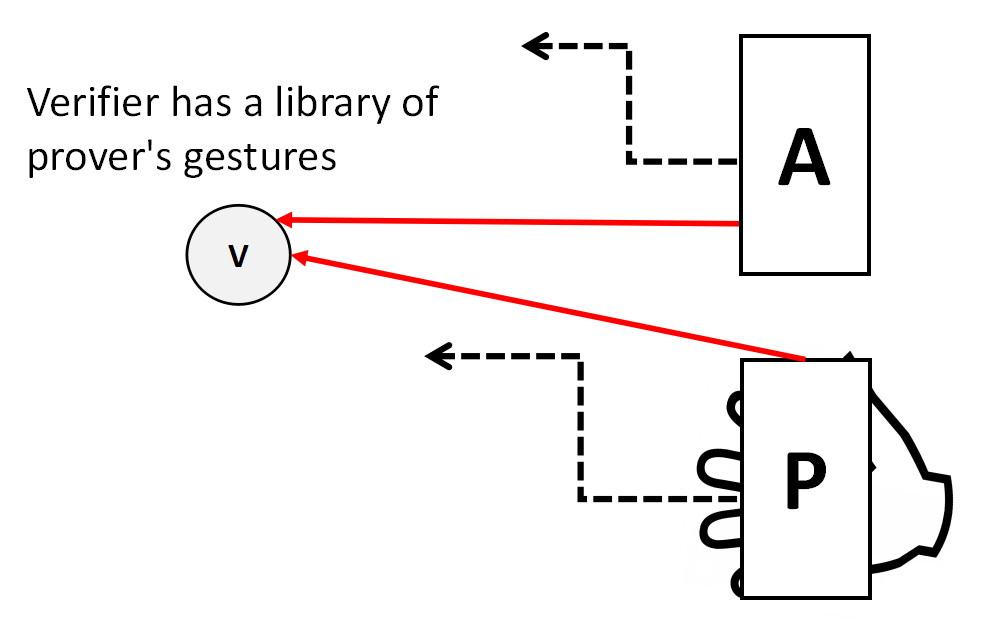
\includegraphics[width=0.65 \linewidth]{./figures/model3.png}
\caption{System model for defense model 3. The verifier (V) and the prover (P) are not synchronized in motion, and the verifier challenges the prover with a series of gestures in its pre-calibrated library. The attacker (A) receives the same prompts, but must mimic what the prover would do for each gesture.}
\label{fig:Model3}
\end{figure}

We hypothesize that there is a inverse correlation between number of gesture challenges and number of false positives (i.e. more challenges reduces the success of an attacker. However, we also hypothesize there is a direct correlation between number of gesture challenges and number of false negatives (i.e. there are more opportunities for the user to fail). We seek to find a threshold that minimizes the number of false positives and false negatives in this model.

%The verifier has a library of gestures previously calibrated by the user. To pair with the verifier, the prover must respond to the verifier's challenge. The verifier will send a gesture image/shape to the prover, and the prover must produce accelerometer data that matches the gesture data at the verifier. 

\end{itemize}

